%  LaTeX support: latex@mdpi.com 
%  For support, please attach all files needed for compiling as well as the log file, and specify your operating system, LaTeX version, and LaTeX editor.

%=================================================================
\documentclass[journal,review,submit,pdftex,moreauthors]{Definitions/mdpi} 

\usepackage{array}
\usepackage{amsmath}
\usepackage{tabularray} % full width tables
\usepackage{rotating} % rotate tables 90'

%--------------------
% Class Options:
%--------------------
%----------
% journal
%----------
% Choose between the following MDPI journals:
% acoustics, actuators, addictions, admsci, adolescents, aerobiology, aerospace, agriculture, agriengineering, agrochemicals, agronomy, ai, air, algorithms, allergies, alloys, analytica, analytics, anatomia, animals, antibiotics, antibodies, antioxidants, applbiosci, appliedchem, appliedmath, applmech, applmicrobiol, applnano, applsci, aquacj, architecture, arm, arthropoda, arts, asc, asi, astronomy, atmosphere, atoms, audiolres, automation, axioms, bacteria, batteries, bdcc, behavsci, beverages, biochem, bioengineering, biologics, biology, biomass, biomechanics, biomed, biomedicines, biomedinformatics, biomimetics, biomolecules, biophysica, biosensors, biotech, birds, bloods, blsf, brainsci, breath, buildings, businesses, cancers, carbon, cardiogenetics, catalysts, cells, ceramics, challenges, chemengineering, chemistry, chemosensors, chemproc, children, chips, cimb, civileng, cleantechnol, climate, clinpract, clockssleep, cmd, coasts, coatings, colloids, colorants, commodities, compounds, computation, computers, condensedmatter, conservation, constrmater, cosmetics, covid, crops, cryptography, crystals, csmf, ctn, curroncol, cyber, dairy, data, ddc, dentistry, dermato, dermatopathology, designs, devices, diabetology, diagnostics, dietetics, digital, disabilities, diseases, diversity, dna, drones, dynamics, earth, ebj, ecologies, econometrics, economies, education, ejihpe, electricity, electrochem, electronicmat, electronics, encyclopedia, endocrines, energies, eng, engproc, entomology, entropy, environments, environsciproc, epidemiologia, epigenomes, est, fermentation, fibers, fintech, fire, fishes, fluids, foods, forecasting, forensicsci, forests, foundations, fractalfract, fuels, future, futureinternet, futurepharmacol, futurephys, futuretransp, galaxies, games, gases, gastroent, gastrointestdisord, gels, genealogy, genes, geographies, geohazards, geomatics, geosciences, geotechnics, geriatrics, grasses, gucdd, hazardousmatters, healthcare, hearts, hemato, hematolrep, heritage, higheredu, highthroughput, histories, horticulturae, hospitals, humanities, humans, hydrobiology, hydrogen, hydrology, hygiene, idr, ijerph, ijfs, ijgi, ijms, ijns, ijpb, ijtm, ijtpp, ime, immuno, informatics, information, infrastructures, inorganics, insects, instruments, inventions, iot, j, jal, jcdd, jcm, jcp, jcs, jcto, jdb, jeta, jfb, jfmk, jimaging, jintelligence, jlpea, jmmp, jmp, jmse, jne, jnt, jof, joitmc, jor, journalmedia, jox, jpm, jrfm, jsan, jtaer, jvd, jzbg, kidneydial, kinasesphosphatases, knowledge, land, languages, laws, life, liquids, literature, livers, logics, logistics, lubricants, lymphatics, machines, macromol, magnetism, magnetochemistry, make, marinedrugs, materials, materproc, mathematics, mca, measurements, medicina, medicines, medsci, membranes, merits, metabolites, metals, meteorology, methane, metrology, micro, microarrays, microbiolres, micromachines, microorganisms, microplastics, minerals, mining, modelling, molbank, molecules, mps, msf, mti, muscles, nanoenergyadv, nanomanufacturing,\gdef\@continuouspages{yes}} nanomaterials, ncrna, ndt, network, neuroglia, neurolint, neurosci, nitrogen, notspecified, %%nri, nursrep, nutraceuticals, nutrients, obesities, oceans, ohbm, onco, %oncopathology, optics, oral, organics, organoids, osteology, oxygen, parasites, parasitologia, particles, pathogens, pathophysiology, pediatrrep, pharmaceuticals, pharmaceutics, pharmacoepidemiology,\gdef\@ISSN{2813-0618}\gdef\@continuous pharmacy, philosophies, photochem, photonics, phycology, physchem, physics, physiologia, plants, plasma, platforms, pollutants, polymers, polysaccharides, poultry, powders, preprints, proceedings, processes, prosthesis, proteomes, psf, psych, psychiatryint, psychoactives, publications, quantumrep, quaternary, qubs, radiation, reactions, receptors, recycling, regeneration, religions, remotesensing, reports, reprodmed, resources, rheumato, risks, robotics, ruminants, safety, sci, scipharm, sclerosis, seeds, sensors, separations, sexes, signals, sinusitis, skins, smartcities, sna, societies, socsci, software, soilsystems, solar, solids, spectroscj, sports, standards, stats, std, stresses, surfaces, surgeries, suschem, sustainability, symmetry, synbio, systems, targets, taxonomy, technologies, telecom, test, textiles, thalassrep, thermo, tomography, tourismhosp, toxics, toxins, transplantology, transportation, traumacare, traumas, tropicalmed, universe, urbansci, uro, vaccines, vehicles, venereology, vetsci, vibration, virtualworlds, viruses, vision, waste, water, wem, wevj, wind, women, world, youth, zoonoticdis 
% For posting an early version of this manuscript as a preprint, you may use "preprints" as the journal. Changing "submit" to "accept" before posting will remove line numbers.

%---------
% article
%---------
% The default type of manuscript is "article", but can be replaced by: 
% abstract, addendum, article, book, bookreview, briefreport, casereport, comment, commentary, communication, conferenceproceedings, correction, conferencereport, entry, expressionofconcern, extendedabstract, datadescriptor, editorial, essay, erratum, hypothesis, interestingimage, obituary, opinion, projectreport, reply, retraction, review, perspective, protocol, shortnote, studyprotocol, systematicreview, supfile, technicalnote, viewpoint, guidelines, registeredreport, tutorial
% supfile = supplementary materials

%----------
% submit
%----------
% The class option "submit" will be changed to "accept" by the Editorial Office when the paper is accepted. This will only make changes to the frontpage (e.g., the logo of the journal will get visible), the headings, and the copyright information. Also, line numbering will be removed. Journal info and pagination for accepted papers will also be assigned by the Editorial Office.

%------------------
% moreauthors
%------------------
% If there is only one author the class option oneauthor should be used. Otherwise use the class option moreauthors.

%---------
% pdftex
%---------
% The option pdftex is for use with pdfLaTeX. Remove "pdftex" for (1) compiling with LaTeX & dvi2pdf (if eps figures are used) or for (2) compiling with XeLaTeX.

%=================================================================
% MDPI internal commands - do not modify
\firstpage{1} 
\makeatletter 
\setcounter{page}{\@firstpage} 
\makeatother
\pubvolume{1}
\issuenum{1}
\articlenumber{0}
\pubyear{2023}
\copyrightyear{2023}
%\externaleditor{Academic Editor: Firstname Lastname}
\datereceived{ } 
\daterevised{ } % Comment out if no revised date
\dateaccepted{ } 
\datepublished{ } 
%\datecorrected{} % For corrected papers: "Corrected: XXX" date in the original paper.
%\dateretracted{} % For corrected papers: "Retracted: XXX" date in the original paper.
\hreflink{https://doi.org/} % If needed use \linebreak
%\doinum{}
%\pdfoutput=1 % Uncommented for upload to arXiv.org

%=================================================================
% Add packages and commands here. The following packages are loaded in our class file: fontenc, inputenc, calc, indentfirst, fancyhdr, graphicx, epstopdf, lastpage, ifthen, float, amsmath, amssymb, lineno, setspace, enumitem, mathpazo, booktabs, titlesec, etoolbox, tabto, xcolor, colortbl, soul, multirow, microtype, tikz, totcount, changepage, attrib, upgreek, array, tabularx, pbox, ragged2e, tocloft, marginnote, marginfix, enotez, amsthm, natbib, hyperref, cleveref, scrextend, url, geometry, newfloat, caption, draftwatermark, seqsplit
% cleveref: load \crefname definitions after \begin{document}

%=================================================================
% Please use the following mathematics environments: Theorem, Lemma, Corollary, Proposition, Characterization, Property, Problem, Example, ExamplesandDefinitions, Hypothesis, Remark, Definition, Notation, Assumption
%% For proofs, please use the proof environment (the amsthm package is loaded by the MDPI class).

%=================================================================
% Full title of the paper (Capitalized)
\Title{Computational approaches and challenges in the analysis of circRNA data}

% MDPI internal command: Title for citation in the left column
\TitleCitation{Title}

% Author Orchid ID: enter ID or remove command
\newcommand{\orcidauthorA}{0000-0002-8492-6585} % Add \orcidA{} behind the author's name
\newcommand{\orcidauthorB}{0000-0002-8628-5814} % Add \orcidB{} behind the author's name
\newcommand{\orcidauthorC}{0000-0002-6702-8564}

% Authors, for the paper (add full first names)
%\Author{Barry Digby $^{1,\dagger,\ddagger}$\orcidA{}, Stephen P. Finn $^{2,\ddagger}$ and Pilib \'{O}Broin $^{1}$*}
\Author{Barry Digby $^{1}$*\orcidA{}, Stephen P. Finn $^{2}$\orcidB{} and Pilib \'{O} Broin $^{1}$\orcidC{}}

%\longauthorlist{yes}

% MDPI internal command: Authors, for metadata in PDF
\AuthorNames{Barry Digby, Stephen Finn, Pilib \'{O} Broin}

% MDPI internal command: Authors, for citation in the left column
\AuthorCitation{Digby, B.; Finn, S.P.; \'{O} Broin, P.}
% If this is a Chicago style journal: Lastname, Firstname, Firstname Lastname, and Firstname Lastname.

% Affiliations / Addresses (Add [1] after \address if there is only one affiliation.)
\address{%
$^{1}$ \quad School of Mathematical and Statistical Sciences, University of Galway, Galway, Ireland \\
$^{2}$ \quad Department of Histopathology and Morbid Anatomy, Trinity Translational Medicine Institute, Dublin, Ireland}

% Contact information of the corresponding author
\corres{Correspondence: b.digby1@universityofgalway.ie}

% Current address and/or shared authorship
%\firstnote{Current address: Affiliation 3.} 
%\secondnote{These authors contributed equally to this work.}
% The commands \thirdnote{} till \eighthnote{} are available for further notes

%\simplesumm{} % Simple summary

%\conference{} % An extended version of a conference paper

% Abstract (Do not insert blank lines, i.e. \\) 
\abstract{Circular RNAs (circRNA) are a class of non-coding RNA, forming a single-stranded covalently closed loop structure generated via back-splicing. 
Advancements in sequencing methods and technologies in conjunction with algorithmic developments of bioinformatics tools have enabled researchers to characterise the origin and function of circRNAs, with practical applications as a biomarker of diseases becoming increasingly relevant. 
Computational methods developed for circRNA analysis are predicated on detecting the chimeric back-splice junction of circRNAs whilst mitigating false-positive sequencing artefacts. In this review, we discuss in detail the computational strategies developed for circRNA identification, highlighting a selection of tool strengths, weaknesses and assumptions. 
In addition to circRNA identification tools, we describe methods for characterising the role of circRNAs within the cometing endogenous RNA (ceRNA) network, their interactions with RNA-binding proteins, and publicly available databases for rich circRNA annotation.}

% Keywords
\keyword{circRNAs; bioinformatics tools; computational challenges; non-coding RNA} 

% The fields PACS, MSC, and JEL may be left empty or commented out if not applicable
%\PACS{J0101}
%\MSC{}
%\JEL{}

%%%%%%%%%%%%%%%%%%%%%%%%%%%%%%%%%%%%%%%%%%
% Only for the journal Diversity
%\LSID{\url{http://}}

%%%%%%%%%%%%%%%%%%%%%%%%%%%%%%%%%%%%%%%%%%
% Only for the journal Applied Sciences
%\featuredapplication{Authors are encouraged to provide a concise description of the specific application or a potential application of the work. This section is not mandatory.}
%%%%%%%%%%%%%%%%%%%%%%%%%%%%%%%%%%%%%%%%%%

%%%%%%%%%%%%%%%%%%%%%%%%%%%%%%%%%%%%%%%%%%
% Only for the journal Data
%\dataset{DOI number or link to the deposited data set if the data set is published separately. If the data set shall be published as a supplement to this paper, this field will be filled by the journal editors. In this case, please submit the data set as a supplement.}
%\datasetlicense{License under which the data set is made available (CC0, CC-BY, CC-BY-SA, CC-BY-NC, etc.)}

%%%%%%%%%%%%%%%%%%%%%%%%%%%%%%%%%%%%%%%%%%
% Only for the journal Toxins
%\keycontribution{The breakthroughs or highlights of the manuscript. Authors can write one or two sentences to describe the most important part of the paper.}

%%%%%%%%%%%%%%%%%%%%%%%%%%%%%%%%%%%%%%%%%%
% Only for the journal Encyclopedia
%\encyclopediadef{For entry manuscripts only: please provide a brief overview of the entry title instead of an abstract.}

%%%%%%%%%%%%%%%%%%%%%%%%%%%%%%%%%%%%%%%%%%
% Only for the journal Advances in Respiratory Medicine
%\addhighlights{yes}
%\renewcommand{\addhighlights}{%

%\noindent This is an obligatory section in “Advances in Respiratory Medicine”, whose goal is to increase the discoverability and readability of the article via search engines and other scholars. Highlights should not be a copy of the abstract, but a simple text allowing the reader to quickly and simplified find out what the article is about and what can be cited from it. Each of these parts should be devoted up to 2~bullet points.\vspace{3pt}\\
%\textbf{What are the main findings?}
% \begin{itemize}[labelsep=2.5mm,topsep=-3pt]
% \item First bullet.
% \item Second bullet.
% \end{itemize}\vspace{3pt}
%\textbf{What is the implication of the main finding?}
% \begin{itemize}[labelsep=2.5mm,topsep=-3pt]
% \item First bullet.
% \item Second bullet.
% \end{itemize}
%}

%%%%%%%%%%%%%%%%%%%%%%%%%%%%%%%%%%%%%%%%%%
\begin{document}

%%%%%%%%%%%%%%%%%%%%%%%%%%%%%%%%%%%%%%%%%%

\section{Introduction}
Originally detected in plant viroids \cite{Sanger1976}, yeast mitochondrial RNA \cite{Arnberg1980Feb} and hepatitis $\delta$ virus \cite{Kos1986Oct}, circRNAs were believed to be discarded intermediates from intron lariat branching or by-products of aberrant splicing \cite{Cocquerelle1993Jan, Qian1992}. During the initial adoption of next-generation sequencing (NGS) technologies, circRNAs remained largely unstudied -- with the poly-A selection protocols in RNA-Sequencing (RNA-Seq) technologies preferentially selecting messenger RNAs (mRNAs). Recent advancements in bioinformatics methods however, coupled with a widening range of protocols to interrogate the transcriptome have enabled the detection of circRNAs, with interest in the field rejuvenated when a landmark study by Salzman et al. (2012) identified RNA transcripts containing `scrambled exons' characteristic of circRNAs in hyperdiploid acute lymphoblastic leukaemia diagnostic bone marrow samples \cite{Salzman2012}. Subsequent studies by Jeck et al. (2012) \cite{Jeck2012Dec}, Hansen et al. (2013), \cite{Hansen2013Mar} and Memczak et al. (2013) \cite{find_circ} identified thousands of circRNAs in metazoans. Moreover, Hansen et al., (2013) \cite{Hansen2013Mar} and Memczak et al. (2013) \cite{find_circ} demonstrated that CDR1as and circSry competitively bind micro RNA (miRNA) sequences via complimentary sites within their mature spliced sequence, suggesting a regulatory role within the competing endogenous RNA (ceRNA) network. These foundational works ushered in a plethora of novel research on circRNAs characterising their origin, biogenesis, structure and functions \cite{Danan2012Apr, Jeck2014May, Ashwal-Fluss2014Oct, Chen2015Apr}. \par

circRNAs exhibit stage and tissue-specific expression \cite{circRNA_finder, Gruner2016, Rybak-Wolf2015Jun} and are enriched in exosomes \cite{Li2015Apr}. Coupled with their high level of stability in contrast to other RNA molecules, circRNAs represent a promising biomarker for disease; circ-ITCH for example, acts as a tumor supressor in lung cancer by inhibiting the Wnt/$\beta$-Catenin pathway \cite{Wan2016}, and circPVT1 acts as an oncogene in head and neck squamous cell carcinoma, displaying overexpression in tumor samples harbouring TP53 mutations \cite{Verduci2017Dec}. In addition to applications as a biomarker, circRNAs can be constructed to target and sequester overexpressed oncogenic miRNAs. The synthetically generated circRNA \textit{CM21D} was produced via t-RNA splicing and administered in experimental glioblastoma models, inhibiting miR-21-5p thus restoring the expression of tumor supressor genes \cite{Bayat2023Jun}. \par

Given their diverse role within cells, it is imperative to accurately identify and annotate the functions of circRNAs using computational methods in conjunction with sequencing data. Multiple bioinformatics tools exist for identifying circRNAs in RNA-Seq datasets via the detection of chimeric reads representative of circRNA back-splice junctions (BSJ). Once a circRNA has been identified, researchers are often interested in quantifying its expression, predicting it's interactions with other small RNAs and RNA binding protiens (RBPs), examining the ratio of circRNA expression compared to its cognate parent gene, and performing differential circRNA expression analyses. In this review, we discuss the current landscape of bioinformatics tools for circRNA analysis encompassing circRNA identification and annotation, circRNA quantification, circRNA functional prediction, and highlight some of the computational challenges involved. Whilst this review focuses on the computational analysis of circRNAs, we briefly detail the origin, biogenesis and structure of circRNAs as this information is necessary for understanding the algorithms employed by circRNA identification tools. For additional details on circRNA biogenesis, degradation, translation, cellular transport, downstream interactions and evolutionary conservation, we direct readers to a selection of recent reviews \cite{Greene2017Jun, Kristensen2019Nov, Li2018Aug, Ren2022Dec, Yang2021May, Huang2020, Panda2018, Santos-Rodriguez2021Sep}. \par

Finally, we also provide an overview of the currently available circRNA databases containing rich annotations for circRNAs derived from various tissue sources and cell lines using RNA-Seq datasets, predicted miRNA and RBP targets using cross-linking and immunoprecipitation sequencing (CLIP-Seq) and circRNAs associated with diseases. 

\begin{figure}
    \begin{center}
        \includegraphics[width=\textwidth]{biogenesis.png}
        \caption{Biogenesis and fucntional mechanisms of circRNAs. \textbf{Nucleus}: circRNA biogenesis via direct back-splicing driven by complementary intronic sequences, RNA-binding proteins or lariat loops containing skipped exons or introns. \textbf{Cytosol}: Cap independent protein translation, RBP binding and miRNA sequestration via complementary miRNA response element sites. \textbf{Plasm}: exosomal circRNAs facilitating non-invasive biomarker discovery.}
        \label{biogen}
    \end{center}
\end{figure}

\section{circRNA biogenesis and structure}
Canonical linear mRNA splicing involves processing precursor mRNA (pre-mRNA) to remove intronic sequences and the joining together of exon sequences to form a mature mRNA transcript. This process is mediated via the spliceosomal machinery composed of small nuclear ribonucleoproteins which recognise conserved 5' splice sites,  3' splice sites and a branch site within the intronic sequence. Spliceosomal machinery binds to the intron's upstream 5' splice donor site, pairing it with the downstream branch site forming a lariat loop structure. Following this, the downstream 3' splice acceptor site of the intron splice site is brought in close proximity to the 3' end of the exon, where, via a process of transesterification, the exons 3' hydroxyl group attacks the phosphodiester bond of the 3' intron splice acceptor site, covalently joining the exons, producing a mature mRNA and releasing the intron lariat structure \cite{BibEntry2019Dec}. \par

circRNA formation relies on canonical splice site signals and spliceosome machinery \cite{Starke2015Jan} however, in contrast to linear RNAs, circRNAs are formed by a process known as back-splicing in which a downstream 5' splice donor site is reversely joined to an upstream 3' splice acceptor site forming a covalently closed loop structure \cite{Jeck2012Dec, Jeck2014May}. This circularization process is mediated by one of three factors (Figure \ref{biogen}):
\begin{itemize}
    \item Intron pairing: RNA pairing across flanking introns in pre-mRNA can occur due to the complementarity of short non-coding \textit{cis} regulatory elements, including repetitive Alu sequences or GU-rich sequences. The pairing forms a hairpin structure that brings the downstream 5' splice acceptor site in close proximity to the upstream 3' acceptor site. This proximity facilitates back-splicing and the formation of exonic circRNAs (EcircRNAs) and exon-intron circRNAs (EIcircRNAs) \cite{Wilusz2015May, Zhang2014Sep}.
    \item RBP pairing: \textit{trans}-factors in pre-mRNA bind to RBP such as Muscleblind (MBNL1) and Quaking (QKI) which in turn bridge flanking introns facilitating back-splicing and the generation of EcircRNAs and EIcircRNAs \cite{Singh2022Jan, Chen2015Apr}.
    \item  Lariat formation: during canonical splicing, an exon-skipping event produces an intermediate lariat containing excised exons and introns. Subsequent internal lariat splicing produces one of a single EcircRNAs \cite{Zaphiropoulos1996} or intronic circRNAs (ciRNAs) \cite{ZHANG2013}.
\end{itemize}

The three categories of circRNAs classes (EcircRNA, EIcircRNA and ciRNA) present diverse internal structures in the final mature spliced sequence: 1) EcircRNAs containing all underlying exons after canonical splicing; 2) alternative EcircRNAs comprised of a subset of underlying exons as a by-product of alternative-splicing; 3) EIcircRNAs composed of both intronic and exonic sequences; and 4) ciRNAs containing intronic sequences. \par

circRNAs` unique covalently closed loop structure lacking 5' and 3' tails confers resistance to RNase R degradation, granting them a much higher half-life than their linear mRNA counterparts \cite{Suzuki2006May, Enuka2016Feb}. This feature makes circRNAs an attractive biomarker in disease-based settings, with reports of circRNAs exhibiting differential expression in gastric, colorectal, ovarian and lung cancers, and enzalutamide resistant LNCaP cell lines \cite{Li2015Apr, Bachmayr-Heyda2015, Lim2021Dec}. Furthermore, circRNAs can be packaged and exported from the cell to bodily fluid via exosomes \cite{Li2015Aug, Shi2020Mar} facilitating the use of non-invasive liquid biopsies to monitor disease progression \cite{Wang2019Feb, Wu2023Apr, Pan2019Nov, Li2020Mar, Chen2020Apr, Louis2019Nov}. The mechanism of circRNA degradation and clearance remains an active area of research. Studies have found that miRNAs can facilitate the degradation of circRNAs via Argonaute 2 (Ago2)-mediated degradation supporting the hypothesis of circRNAs as active members in the ceRNA network \cite{Hansen2011Sep}. Other works demonstrate RNase H1-mediated degradation of ciRNAs with high GC content \cite{Li2021Nov} and the degradation of circRNAs containing m\textsuperscript{6}A modifications via endoribonucleolytic cleavage \cite{Park2019May}. 

\section{Principles and challenges for circRNA identification}

\begin{figure}
    \begin{center}
        \includegraphics[width=\textwidth]{artefacts.png}
        \caption{Advancements in biochemical and bioinformatics strategies for circRNA detection. \textbf{Library preparation}: Left to right, in order of increasing circRNA sensitivity; polyA(+): unsuitable for circRNA detection, preferentially selects mRNAs; rRNA(-): ribosomal RNA depletion yielding a library with circRNAs and mRNAs; rRNA(-) \& polyA(-): ribosomal RNA depletion in conjunction with polyadenylation and depletion of polyA transcripts; rRNA(-) \& RNase R(+): ribosomal RNA depletion in conjunction with RNase R ribonuclease treatment depleting mRNAs; RPAD: RNase R treatment followed by polyadenylation and polyA\textsuperscript RNA depletion, yielding a highly pure circRNA library. \textbf{Alignment strategies}: Unmapped reads to the reference genome can be used to perform split alignment to identify reads aligning in opposite directions, or to map reads to  a BSJ pseudo-reference. \textbf{Validation strategies}: Paired-end sequencing greatly reduces false-positives, mates that map across the BSJ whose mates reside within the same transcript are indictive of circRNAs.}
        \label{artefacts}
    \end{center}
\end{figure}

\subsection{Library preparation}
circRNAs represent approximately 1-3\% of the transcriptome pool in total RNA sequencing libraries \cite{Guria2022May}, dictating novel strategies to enrich circRNA libraries prior to sequencing (Figure\ref{artefacts}). A typical eukaryotic RNA-Seq library preparation protocol involves the preferential selection of RNAs with polyA tails or the depletion of ribosomal RNAs (rRNAs). Due to circRNAs' covalently closed loop structure, polyA selection in libraries will almost completely remove all circular transcripts in a sample. By contrast, circRNAs are retained in rRNA-depleted samples and are enriched in samples treated with ribonuclease R (RNase R) to deplete linear RNAs. Random priming is preferred to oligo(dT) priming, as the former generates random oligonucleotide sequences for cDNA synthesis independent of polyA sequences, whilst the latter will generate libraries biased towards linear RNAs. One method, termed "RNase R treatment followed by polyadenylation and polyA\textsuperscript{+} RNA depletion" (RPAD) has emerged as a leading candidate for circRNA library preparation yielding the highest number of circRNAs and the highest sensitivity in a benchmark study \cite{Shi2022Dec}. RPAD employs the sequential depletion of linear RNAs via RNase R treatment, polyadenylation of remaining linear RNAs and a final round of polyA\textsuperscript{+} depletion using oligo(dT) beads followed by ribosomal RNA (rRNA) depletion to yield a high concentration circRNA library for sequencing \cite{Panda2017Jul, Pandey2019Feb}. In the absence of the RPAD method, rRNA depletion or RNase R\textsuperscript{+} are sufficient for generating RNA-Seq datasets for circRNA detection and have been used in benchmark studies analysing the performance of circRNA identification tools \cite{DCC}.

\subsection{Sequencing artefacts}
Technical artefacts introduced during sequencing can lead to the generation of false positives during circRNA identification. Reverse transcriptase, an enzyme used to synthesise complementary cDNA strands can undergo a template-switching event when brought in close proximity to a different RNA template with a suitable region for priming \cite{Cocquet2006Jul}. The original, incomplete synthesized strand is carried to the newly 'switched` cDNA template where reverse transcriptase continues generating a chimeric molecule capable of mimicking alternative splicing and backsplicing. Alarmingly, these template switching events can account for up to 35-55\% of the isoforms computationally detected for a gene \cite{Roy2015}. Sequencing libraries that use adapter-ligation steps are at risk of generating chimeric sequences -- albeit at a much lower level. Finally, incorrectly called bases at the beginning or end of exons in genes containing highly homologous sequences can generate false positive splice site signals (GU/AG, etc.) \cite{Salzman2014Jun}. With respect to circRNAs, these sequencing errors can lead to sites that are mistakenly identified as backsplice sites when identifying circRNAs in samples. Due to the low levels of circRNA expression in cells when compared to other RNA transcripts, the presence of sequencing artefacts cannot be overcome by simply applying a read depth filter to quantification results. circRNA identification tools typically require paired-end data to overcome this source of error by requiring read 1 to map to the back-splice junction (BSJ) and its corresponding read 2 pair to map in the same transcript within a fixed distance \cite{Salzman2012}.

\subsection{BSJ-based circRNA identification}
The main step of any circRNA analysis is the identification of circRNAs in RNA-Seq datasets. This analysis is predicated on the detection of the BSJ, i.e the scrambled exon junctions representing the joining of an upstream 5' donor site to the downstream 3' acceptor site to form a circular structure. The majority of circRNA identification tools can be classed as one of two sub-groups: segmented-based-approach, whereby anchors (fixed-length segments taken from the end of reads) are extracted from unmapped sequencing reads and re-mapped to the genome; or pseudo-reference based in which a custom database of manually curated BSJ sites are generated and used to map the sequencing reads (Figure\ref{artefacts}). The first strategy allows for \textit{de novo} circRNA identification whilst the second is constrained to exons contained within the reference annotation file used for constructing the pseudo-reference database. As circRNA identification tools evolved, developers began to blend the two approaches to optimize the process of circRNA identification. \par
The first circRNA identification analysis performed by Salzman et al. (2012) \cite{Salzman2012} used the pseudo-reference based approach to identify circRNAs in ALL samples. Reads that mapped contiguously to RefSeq annotated genes using Bowtie \cite{Bowtie} were considered representative of linear transcripts and removed from the analysis. Subsequently, the RefSeq database was used to create a custom database of all intragenic exon-exon junctions against which reads that failed to align were mapped. An exon scrambling event was flagged if read 1 mapped to a non-canonical exon-exon junction as defined by the custom RefSeq database and read 2 mapped within the same transcript. The number of reads spanning the scrambled exon junction was used to estimate the relative abundance of candidate circRNAs. In contrast to the pseudo-reference based approach, the first tool created for the purpose of circRNA detection `find\_circ' \cite{find_circ} utilises the segmented-based approach. Firstly, paired-end reads are aligned to the genome to extract reads that do not contiguously align. A customised script then splits unmapped reads to obtain 20 nucleotide anchor sequences originating from the 5` and 3` ends of the reads. The anchors are re-aligned to the genome, with anchors mapping in reverse orientation extended to identify the breakpoint site in the anchor. The resulting BED file is filtered using the following criteria to arrive at a set of circRNAs: 1) splice sites must be flanked by GU/AG signals; 2) unambivalant breakpoints; 3) less than 2 mismatches in the extension procedure; 4) breakpoint cannot reside more than 2 nucleotides inside the anchor; 5) more than 2 reads must support the BSJ site and 6) splice sites must not be more than 100Kb apart. \par
UROBORUS \cite{UROBORUS} adopts a similar approach to `find\_circ', collecting and extracting 20bp anchors from reads that failed to map contiguously to the reference genome using TopHat. Anchor segments representative of a circRNA BSJ site mapped in reverse orientation within the same transcript with an overhang of $>$20bp at either end of both segments are termed `balanced mapped junctions' (BMJ) whilst segments with an overhang $<$20bp in one read are termed `unbalanced mapped junctions' (UMJ) and subject to different extension strategies. Both BMJ reads are separately extended outwards to the nearest splice-site to form paired-end segments, whilst for UMJ reads, the shorter mate is discarded and the single mapped seed is outwardly extended to the nearest splice-site (an extension distance must not exceed the length of the read minus 3bp). Bowtie is then used to remap the paired-end and single extended segments; segments aligning to the reference genome in the opposite orientation with read support $>$2 as detected by the UROBORUS algorithm are representative of circular candidates. \par
Post-transcriptional exon shuffling finder (PTESfinder) \cite{PTESfinder} combines the segment-based approach with the pseudo-reference based approach to identify circular candidates using Bowtie. Briefly, 20bp segment anchors are extracted from the ends of input sequencing reads and mapped to the reference transcriptome. Anchors that map to the same gene but in an inverted orientation are identified and used to construct a pseudo-reference (termed `PTES constructs') by concatenating the last 65bp of the underlying 5' exon and the first 65bp of the 3' exon. Reads are then aligned to the PTES construct, as well as genomic and transcriptomic references in order to generate mapping scores for circular candidate filtering. Candidates are marked as circRNAs when they exhibit high mapping scores to the PTES construct and low scores to the genomic and transcriptome reference. \par 
The concept of mapping reads to genomic, transcriptomic and BSJ databases to filter circRNA candidates was further improved upon by KNIFE \cite{KNIFE}. KNIFE maps reads to rRNA sequences, genomic, transcriptomic and a customised BSJ reference database using Bowtie2, discarding candidates that map with high scores to databases other than the custom BSJ reference. Where paired-end RNA-Seq data is available, the candidate reads spanning the BSJ site are subsetted into circRNA and decoy reads based on mapping information available in order to mitigate against false-positive BSJ reads generated by sequencing errors. For reads that fail to map to any of the databases, a \textit{de novo} analysis is performed using Bowtie coupled with a segment-based approach whereby segments are used to construct a \textit{de novo} index. The unmapped reads are then re-aligned to the \textit{de novo} index using Bowtie2 with the same criteria for pseudo-reference based alignment. KNIFE is one of the first circRNA identification tools to employ a statistical framework by obtaining a posterior probability for each circRNA candidate to predict if it is a true positive by using a logistic generalized linear model (GLM) based on the alignment features of read 1. In contrast to the circRNA identification tools discussed thus far which require extracting anchor sequences to identify putative BSJ sites using Bowtie or Bowtie2, both BWA and STAR are capable of directly detecting breakpoint events and chimeric fusions during read alignment. circRNA identification tools utilizing BWA or STAR therefore circumvent the need to manually extract anchors for BSJ identification using customized scripts, streamlining the process of circRNA identification and reducing computational overheads. \par 
CircRNA Identifier (CIRI) \cite{CIRI} is one such tool that utilises BWA-MEM sequence alignment mapping (SAM) information to identify reads in which two segments of the read align in chiastic order termed `paired chiastic clipping' (PCC) signals. Subsequent filtering leveraging paired-end mapping (PEM) information, GU/AG splice signals and mapping rates to homologous sequences removes false positives to arrive at a set of high-confidence circRNAs. One shortcoming of CIRI is its handling of unbalanced junction reads. Unbalanced junction reads are segments of length $<$19bp which are ignored by BWA-MEM to prevent multi-mapping and erroneous mapping, therefore lacking the necessary alignment information in the SAM file for CIRI to detect PCC signals. CIRI uses a dynamic programming algorithm to re-map unbalanced junction reads to balanced junction reads originating from the same junctions detected in the first alignment step. This step is computationally expensive and leads to the generation of false positives, an area specifically addressed by its successor, CIRI2 \cite{CIRI2}. CIRI2 is more cautious when addressing unbalanced junction reads and balanced junction reads with low mapping quality by utilising a maximum likelihood estimation (MLE) based on multiple seed matching. The undetermined segment of a putative BSJ read is divided into \textit{n} seeds of length \textit{m} (for example, a 50bp segment divided into five seeds of length 10bp) to determine if the segment belongs to a forward splice region or a back-splice region. The matched-seed numbers derived from the back-splice region ($k$\textsubscript{1}) and the forward-splice region ($k$\textsubscript{2}) are compared to produce two possible results $k$\textsubscript{1}$>$$k$\textsubscript{2}$=$ back-splice region; $k$\textsubscript{1}$\leq$$k$\textsubscript{2}$=$ forward-splice region. Since its publication in 2018, CIRI2 has become one of the most popular circRNA identification tools and has since been subsumed by CIRIquant \cite{CIRIquant} which extends its functionality by creating a pseudo-reference based on circular candidates detected by CIRI2, against which candidate reads are re-aligned using HISAT2. In addition to improved alignment, CIRIquant performs RNase R correction, linear RNA quantification, and automated differential expression analysis of circRNAs. ACFS \cite{ACFS} is another identification tool that uses BWA, however, its approach to circRNA identification is somewhat unorthodox. ACFS converts paired-end data to single-end data and collapses the reads prior to alignment, borrowing a strategy commonly used for miRNA alignment and quantification. After identifying candidate reads containing segments mapping in inverse orientation, ACFS uses maximum entropy models to predict the underlying BSJ sequence most likely to be generated by splicing. The advantage of this approach is that non-canonical dinucleotide splice sites are considered. The authors also point to the tool's ability to detect fusion circRNAs generated by chromosomal translocation events. This raises the question as to how ACFS controls for sequencing artefacts which can mimic fusion events - particularly when the tool discards paired-end read information. \par
circRNA\_finder \cite{circRNA_finder} and CIRCexplorer \cite{CIRCexplorer} were the first tools to use the outputs from the STAR aligner to identify circRNAs. STAR is capable of directly detecting and writing chimeric reads to the output binary alignment map (BAM) file or separately to a junctions.out tab-separated text file when `--chimSegmentMin' is set to a positive integer. Both circRNA\_finder and CIRCexplorer take advantage of the lightweight junctions.out file which contains within each line the genomic coordinates and CIGAR flags corresponding to each read segment that comprise the chimeric RNA molecule. circRNA\_finder imposes filtering on the putative circRNAs, allowing at most 3 mismatches, uniquely mapped reads, a maximum distance between splice-donor sites of 100kb and the condition that if one read spans the BSJ site, its mate should reside within the interval between the splice donor and acceptor site. Interestingly, CIRCexplorer does not impose such filtering strategies. It instead benefits from using an input reference gene annotation file to annotate putative circRNAs, thereby constraining results to exon-exon boundaries contained within the reference file, reducing the rate of false-positives. CIRCexplorer was superseded by CIRCexplorer2 \cite{CIRCexplorer2}, adding a suite of new modules for circRNA identification including alignment using TopHat-Fusion, annotation of circRNAs, \textit{de novo} assembly of novel circRNAs, characterising alternative-splicing events within circRNAs and support for parsing BWA, MapSplice, STAR and Segemehl outputs. The deprecation of TopHat and TopHat-Fusion has resulted in CIRCexplorer2 largely becoming a tool for the downstream parsing and annotation of outputs from BWA, MapSplice, Segemehl and STAR. DCC \cite{DCC} is yet another circRNA identification tool that harnesses the power of the STAR aligner. In its recommended workflow, paired-end mates are mapped using STAR and each individual mate is processed in the same manner, generating three output files per sample -- joint mapping, mate1 and mate2 junctions.tab files. DCC also offers a junction ratio test using CircTest to formally test variation in expression between circRNAs and their parent gene. We have noted that the sensitivity of circRNA identification tools using STAR can be drastically increased by implementing STAR 2-Pass mode, in which the chimeric junctions detected in all samples during the first mapping stage can be collected and incorporated into the reference genome on the fly during the second pass mapping stage for a sample. This method comes at the cost of increased false positives \cite{Engstrom2013Dec} and as such we recommend users adopt an ensemble approach or set suitably strict filtering parameters on detected circRNAs when employing STAR 2-Pass mode with circRNA\_finder, CIRCexplorer2 or DCC. \par
Finally, there exist splice-aware aligners that are capable of directly handling unmapped reads for detecting circRNAs during the alignment step. Non-co-linear scan (NCLscan) \cite{NCLscan} and segemehl \cite{segemehl} are two popular tools for this task, however, as NCLscan uses the proprietary aligner Novoalign, it's use is dependent on an active Novocraft membership. For this reason segemehl is considered the more popular tool in academic circles and has been incorporated into CIRCexplorer2 and intergration-based tools. 

\subsection{Integration-based identification methods}
A study by Hansen et al. (2016) \cite{Hansen2016Apr} highlighted the discrepancies in results generated by the most popular circRNA identification tools at the time (circRNA\_finder, CIRCexplorer, CIRI, find\_circ and MapSplice). Strikingly, only 854 circRNAs were identified by all tools out of the 5071 unique circRNAs detected, indicating that the choice of circRNA identification tool drastically impacts analyses. Furthermore, the use of RNase R\textsuperscript{+} and RNase R\textsuperscript{-} libraries from the same samples permitted the calculation of false positives returned by each tool. By analysing each paired combination of circRNA identification tools, the authors show that CIRCexplorer + CIRI had the highest rate of false positives (10.76\%), whilst circRNA\_finder + MapSplice achieved the lowest false-positive rate amongst analysed pairs (8.3\%). Perhaps the biggest takeaway from the study was that the combination of all tools yielded a false positive rate of 6.56\%, trading increased precision at the cost of reduced sensitivity. In 2018 Hansen \cite{Hansen2018} performed the same analysis again, this time using 11 circRNA identification tools (ACFS, CIRCexplorer, CIRCexplorer2, CIRI, CIRI2, DCC, find\_circ, KNIFE, MapSplice and UROBORUS). Results echoed those from 2016, with Hansen providing the following key recommendation when adopting an ensemble approach: users should combine results from circRNA identification tools that utilise different aligners to avoid biases. One such example is circRNA\_finder and DCC, which both use the STAR aligner. These two algorithms are thus less suited for pairing as the false positives generated are likely to be inherent to the aligner used. The analyses performed by Hansen et al. set new standards for best practices surrounding circRNA detection, ushering in a new class of circRNA identification pipelines termed `integrated tools' in which the user can select one or multiple tools for circRNA identification analysis with an automated intersection of results based on user-defined parameters. \par
CircomPara, developed by Gaffo et al. (2017) \cite{CirComPara} represents the first integration-based identification tool offering users the choice of CIRI, CIRCexplorer (STAR, BWA or Segemehl) and find\_circ. Results are configurable by requiring detected circRNAs to have \textit{n} reads spanning their BSJ site or circRNAs to be called by at least \textit{n} tools. Requiring only input sequencing reads, a reference FASTA file and a reference annotation file, the workflow streamlines the process of circRNA identification for users by automatically generating the required genome indices, reformatting reference annotation files and executing scripts for the analysis. The authors have also made the considerable effort to create a docker container with all of the necessary software for the analysis included, circumventing the need to install any tools from source. Gaffo et al. made substantial upgrades to CircomPara in 2022 by releasing CircomPara2 \cite{CirComPara2}. In addition to offering updated circRNA identification tools to the user (CIRI2, CIRCexplorer2 (BWA, Segemehl, STAR, TopHat), DCC and find\_circ), the workflow includes an improved expression estimate step when consolidating results from multiple tools. In CircomPara, circRNA abundances from multiple methods were calculated using the median of library-normalized BSJ counts across tools. In CircomPara2, the authors identify, for each method, the number of unique reads spanning the BSJ site of a circRNA thereby preserving the information returned by each tool used. Similar to CircomPara, CircomPara2 is packaged in a docker container facilitating rapid execution for users. \par
Several other integration tools exist for circRNA identification \cite{circRNAwrap, DEBKS, circmeta, circRNAprofiler, FcircSEC}, however they operate by using as input previously generated results from circRNA identification tools, unlike CircomPara and CircomPara2 which produce results directly from raw sequencing reads. Another novel integration tool that works with raw sequencing data is nf-core circrna, a workflow for the quantification, miRNA target prediction and differential expression analysis of circRNAs \cite{Digby2023Dec}. The workflow takes as input raw sequencing reads, a reference FASTA, reference gene annotation file and performs all of the preprocessing steps and execution scripts required for a circRNA analysis using circRNA\_finder, CIRIquant, CIRCexplorer2 (STAR), DCC, find\_circ, MapSplice and Segemehl. Similarly to CircomPara, the user can specify custom filtering parameters dictating the intersection strategies used on results. With support for 18 species, the workflow additionally performs automatic miRNA target prediction using miRanda and TargetScan, and automated differential expression analysis of circRNAs between phenotypes of interest provided in an optional metadata file. Developed using nextflow DSL2, the workflow requires Java version $>$8, the latest version of nextflow and a container client which will automatically download software packages for each analysis step (Docker, Apptainer, Conda) facilitating rapid `out-of-the-box' deployment using a single command.

\subsection{Full circle reconstruction} \label{Full circle reconstruction}
The first iteration of circRNA detection tools discussed above are predicated on identifying circRNAs via the presence of BSJ reads in sequencing data. Whilst this is an effective method to detect and quantify circRNAs in RNA-Seq data, the underlying mature spliced sequence (i.e the internal structure) of circRNAs remained opaque. circRNAs are subject to internal splicing events and intron retention (EIcircRNAs), therefore assuming that all of the underlying exons are retained within a circRNA will lead to false positives when predicting their targets based on sequence alignment against miRNA and RBP databases. To overcome this limitation and elucidate circRNA isoforms, coverage of paired-end RNA-Seq reads through the circRNA are utilised to characterise read densities amongst exons within the circular transcript. Full characterization of circRNAs (FUCHs) \cite{FUCHS} was the first tool released capable of delineating circular isoforms, accepting as input results from  circRNA\_finder, CIRI2, CIRCexplorer2, and DCC in conjunction with a BAM file containing chimeric reads, linear reads and unmapped reads. The first step is to isolate circular reads from the BAM file, then identify splicing events within the circular transcript by detecting exon-skipping events in reads. The coordinates of the skipped exons are used to generate coverage statistics, assigning reads to one of two circular isoforms. The output files generated detail the circular candidate's genomic location coupled with read depth for each underlying exon. In this way, researchers can delineate the spliced transcript by removing exons with a read count of 0. The developers of CIRI2 have developed the software package CIRI-AS \cite{CIRI-AS} for \textit{de novo} detection of circRNA exons. Using the outputs from CIRI2 and a BAM file generated by BWA-MEM, the algorithm works by analysing local alignment positions of segments within candidate BSJ reads and its paired mate to identify forward spliced junctions representative of joined circular exons. For each circexon candidate, sequencing depth variation, BSJ read pair coverage and splice junctions from non-BSJ reads are taken into account. CIRI-AS can be performed without a reference GTF file, permitting flexible usage with non-reference organisms. In addition to detecting circexons, CIRI-AS can detect intronic or intergenic circRNA fragments (ICFs) when adequate sequencing depth is provided. CIRI-full \cite{CIRI-full} is yet another tool for full resolution of circRNAs internal structure developed by the same group. The main premise of CIRI-full revolves around the detection of reverse overlap (RO) reads. During reverse transcription, the circular structure of circRNAs can cause continuous circumnavigation of reverse transcriptase within the circRNA, producing read pairs that overlap in reverse orientation. Moreover, the presence of a 3'-RO overlap in both RO reads indicates the full circle has been transcribed facilitating full circRNA reconstruction. For RO reads that do not overlap due to insert size length, CIRI-full borrows information from CIRI2 (BSJ sites) and CIRI-AS (circexons) to produce a reconstructed circRNA. Next, a forward-splice graph (FSG) is constructed by assembling BSJ and RO reads within a detected circRNA BSJ site to model the read coverage of each path using Monte Carlo simulations, providing resolution of circRNA isoforms. 

\subsection*{Machine learning circRNA identification}
circRNA biogenesis can be attributed to hallmarks within the mature sequence and the flanking regions: homologous sequences in flanking introns \cite{Ivanov2015Jan}, inverted repeats \cite{Dubin1995Dec}, the presence of ALU/tandem repeats \cite{Jeck2012Dec} and the density of single nucleotide polymorphisms (SNP) \cite{Thomas2014Aug}. These hallmarks coupled with evolutionary conservation and secondary structure have been identified as the top ranking features for discriminating circRNAs from other classes of lncRNAs using statistical and machine learning (ML) based approaches (minimum redundancy maximum relevance (mRMR) method \cite{Chen2018Feb}, Random Forest, LightGBM, XGBoost \cite{StackCirRNAPred} and multiple kernel learning \cite{PredcircRNA}). A limitation of these methods is that splice site and back-splice junctions are ignored, focusing instead on sequence context. Given the unique BSJ of circRNAs, it is key to understand the properties and relationships between splice sites that constitute canonical linear splicing and a circular back-splicing event. circDeep \cite{circDeep} and DeepCirCode \cite{DeepCirCode} analyzes the nucleotide sequences of two splice sites and model the flanking regions to predict circRNAs by leveraging sequences from circBase and circRNADb in conjunction with deep learning models. Junction encoders and deep interation (JEDI) among splice sites \cite{JEDI} is a tool that optimizes a deep learning model for circRNA prediction in the absence of annotated back-splice sites as training data (zero-shot learning). Unlike its predecessors, JEDI is not limited to interrogating only two splice sites. In this way, it can model the sequence context and flanking regions of all splice sites within an transcript, making it an effective tool for classifying circRNAs that are derived from genes which also produce linear transcripts.




\begin{adjustwidth}{-\extralength}{0cm}
\begin{longtblr}[
        caption = {Bioinformatic tools for circRNA identfication, quantification, isoform detection, full circle reconstruction, target prediction and differential expression analysis.},
        label = {circtools},
        note{\textsuperscript{*}} = {\textit{DEA} = Differential expression analysis},
        note{\textsuperscript{**}} = {\textit{Manual}, requires one of source installation from GitHub, compilation using make, prerequisite software to be previosuly installed or a combination of all three. \textit{BioContainers}, all Conda packages are automatically converted to container images hosted on \href{https://biocontainers.pro/}{BioContainers}. Available via container clients such as singularity, docker etc.},
        note{\textsuperscript{***}} = {\textit{NA} refers to downstream tools that consume previously generated circRNA identififcation tool outputs as input, or classification tools that leverage experimentally validated interactions for prediction tasks.}
        ]{
        colspec = {lX[4]X[1.3]X[1]Xr} %% put weights for column width in [] 
        }
        \hline
        \textbf{Tool name} & \textbf{Description}\textsuperscript{*} & \textbf{Installation}\textsuperscript{**} & \textbf{Aligner}\textsuperscript{***} & \textbf{Language} & \textbf{Ref} \\
        \hline
        \href{https://github.com/arthuryxt/acfs}{ACFS} & Identification \& quantification of circRNAs & Manual & BWA, BLAT & Perl & \cite{ACFS} \\
        \href{https://github.com/tgen/ACValidator}{ACValidator} & Assembly based circRNA detection & Manual, pip & BWA, Bowtie2 & Python2 & \cite{ACValidator} \\
        \href{https://annogesic.readthedocs.io/en/latest/}{ANNOgesic} & Archael/bacterial circRNA identification & Manual, pip3, Docker & segemehl & Python3 & \cite{ANNOgesic} \\
        \href{https://github.com/chanzhou/AutoCirc}{AutoCirc} & Fast identification of circRNAs & Manual & Bowtie2 & C++,Perl & \cite{AutoCirc} \\
        \href{https://github.com/pmenzel/biq}{BIQ} & Identify circRNAs using k-mers spanning BSJ & Manual & k-mer & C++,Perl, JavaScript & \cite{BIQ} \\
        \href{https://github.com/xiaofengsong/CircAST}{CircAST} & Full circle reconstruction, assemble \& quantify circular isoforms & Manual & TopHat & Python2 & \cite{CircAST} \\
        \href{https://github.com/lxwgcool/CircDBG}{CircDBG} & De Bruijn graph detection of circRNAs & Manual & k-mer & C++ & \cite{CircDBG} \\
        \href{https://github.com/UofLBioinformatics/circDeep}{circDeep} & circRNA ifdentification using deep learning & Manual & k-mer & Python3 & \cite{circDeep} \\
        \href{https://github.com/YangLab/CIRCexplorer}{CIRCexplorer} & Identify, quantify \& annotate circRNAs & Conda, pip, BioContainers & {STAR,\\TopHat} & Python2 & \cite{CIRCexplorer} \\
        \href{https://github.com/YangLab/CIRCexplorer2}{CIRCexplorer2} & Identify, quantify \& annotate circRNAs with updated \textit{De novo} module & Conda, pip, BioContainers & BWA, MapSplice, Segemehl, STAR, TopHat & Python2 & \cite{CIRCexplorer2} \\
        \href{https://github.com/YangLab/CLEAR}{CIRCexplorer3} & Compare circRNA \& linear expression & Manual & Hisat2, StringTie & Python3 & \cite{CIRCexplorer3} \\
        \href{https://github.com/yangence/circfull}{circfull} & Detect circRNA isoforms from nanopore reads & Manual & minimap2 & Python3 & \cite{circfull} \\
        \href{https://github.com/Peppags/circLGB-circMRT}{circLGB-circMRT} & Predicting circRNA regulatory interactions by machine learning & Manual & \textit{NA} & Python2 & \cite{circLGB-circMRT} \\
        \href{https://github.com/lichen-lab/circMeta}{circMeta} & Downstream functional analysis of circRNAs & devtools & \textit{NA} & R & \cite{circmeta} \\
        \href{https://github.com/lxwgcool/CircMarker}{CircMarker} & Fast identification of circRNAs & Manual & k-mer & C++, JavaScript & \cite{CircMarker} \\
        \href{https://github.com/egaffo/CirComPara}{CircomPara} & Automated detection of circRNAs usign integrated approach & Manual, Docker & Multiple & Python2, R & \cite{CirComPara} \\
        \href{https://github.com/egaffo/CirComPara}{CirComPara2} & Automated detection of circRNAs using integrated approach & Manual, Docker & Multiple & Python2, R & \cite{CirComPara2} \\
        \href{https://bis.zju.edu.cn/CircPro/}{CircPro} & circRNA coding potential using RNA-Seq \& Ribo-Seq reads & Manual & BWA & Perl & \cite{CircPro} \\
        \href{https://github.com/orzechoj/circRNA_finder}{circRNA\_finder} & Identification of circRNAs & {Conda,\\BioContainers} & STAR & Perl & \cite{circRNA_finder} \\
        \href{https://github.com/duolinwang/CircRNAFisher}{circRNAFisher} & Identification of circRNAs using statistical framework & Manual & Bowtie2 & Perl & \cite{circRNAFisher} \\
        \href{https://bioconductor.org/packages/release/bioc/html/circRNAprofiler.html}{circRNAprofiler} & Downstream functional analysis of circRNAs & BiocManager & \textit{NA} & R & \cite{circRNAprofiler} \\
        \href{https://github.com/liaoscience/circRNAwrap}{circRNAwrap} & Automated detection, abundance, isoform \& DE analysis & Manual & Multiple & UNIX & \cite{circRNAwrap} \\
        \href{https://jakobilab.org/research/circtools/}{circtools} & Suite of tools to identify, quantify, visualise \& perform DEA & Docker, pip3 & STAR & Python3,R & \cite{circtools} \\
        \href{https://sourceforge.net/projects/ciri/files/}{CIRI} & Identification \& quantification of circRNAs & Manual & BWA & Perl & \cite{CIRI} \\
        \href{https://sourceforge.net/projects/ciri2/files/}{CIRI2} & Identification \& quantification of circRNAs & Manual & BWA & Perl & \cite{CIRI2} \\
        \href{https://sourceforge.net/projects/ciri/files/CIRI-AS/}{CIRI-AS} & Alternative circRNA splicing & Manual & BWA & Perl & \cite{CIRI-AS} \\
        \href{https://sourceforge.net/projects/ciri/files/CIRI-full/}{CIRI-full} & Full circle reconstruction & Manual & BWA & JavaScript & \cite{CIRI-full} \\
        \href{https://sourceforge.net/projects/ciri/files/CIRI-long/}{CIRI-long} & Identify circRNAs in Nanopore reads  & Manual & {BWA,\\minimap2} & C++, Python3 & \cite{CIRIlong} \\
        \href{https://sourceforge.net/projects/ciri/files/CIRIquant/}{CIRIquant} & Identification, quantification, RNAase R correction, DEA of circRNAs & Manual & BWA, HISAT2 & Perl & \cite{CIRIquant} \\
        \href{https://sourceforge.net/projects/ciri/files/CIRI-viz/}{CIRI-viz} & Visualising circRNA alignments \& isoforms & Manual & \textit{NA} & JavaScript & \textit{NA} \\
        \href{http://www.bioinformatics.team}{CirRBP} & Stacked generalization ensemble deep learning model to identify RBP binding sites & Web server & \textit{NA} & \textit{NA} & \cite{CirRBP} \\
        \href{http://server.malab.cn/CirRNAPL/}{CirRNAPL} & circRNA identification using machine learning & Web server & \textit{NA} & \textit{NA} & \cite{CirRNAPL} \\
        \href{https://github.com/kavin525zhang/CRIP}{CRIP} & Predict circRNA-RBP interactions using neural networks \& stacked codon-encoding & Manual & \textit{NA} & Python3 & \cite{CRIP} \\
        \href{https://github.com/stiv1n/CYCLeR}{CYCLeR} & Reconstruct \& quantify circRNAs & Docker & BWA, STAR, kallisto & R & \cite{CYCLeR} \\
        \href{https://github.com/dieterich-lab/DCC}{DCC} & Identify \& quantify circRNAs & {Conda,\\BioContainers} & STAR & Python2 & \cite{DCC} \\
        \href{https://github.com/yangence/DEBKS}{DEBKS} & Downstream differential circRNA analysis & Conda, pip & \textit{NA} & Python3 & \cite{DEBKS} \\
        \href{https://github.com/BioDataLearning/DeepCirCode}{DeepCirCode} & circRNA ifdentification using deep learning & Manual & \textit{NA} & Pyton2, R & \cite{DeepCirCode} \\
        \href{https://github.gersteinlab.org/exceRpt/}{exceRpt} & extracellular circRNA profiling & Manual, Docker & Bowtie2, STAR & JavaScript, UNIX & \cite{exceRpt} \\
        \href{https://github.com/tofazzal4720/FcircSEC}{FcircSEC} & Full sequence reconstruction & {CRAN,\\devtools} & \textit{NA} & R & \cite{FcircSEC} \\
        \href{https://github.com/marvin-jens/find_circ}{find\_circ} & Identification \& quantification of circRNAs & {Conda,\\BioContainers} & Bowtie2 & Python2 & \cite{find_circ} \\
        \href{https://github.com/dieterich-lab/FUCHS}{FUCHS} & Alternative circRNA splicing & Manual & \textit{NA} & Python2, R & \cite{FUCHS} \\
        \href{https://github.com/NextGenBioinformatics/hppRNA}{hppRNA} & Workflow for mRNA, lncRNA, circRNA identification \& quantification & Manual & STAR & Perl & \cite{hppRNA} \\
        \href{https://github.com/Xinglab/isoCirc}{isoCirc} & Full length circRNA isoform reconstruction & Manual, pip & Minimap2 & \cite{isoCirc} \\
        \href{https://github.com/hallogameboy/JEDI}{JEDI} & circular RNA prediction based on junction encoders and deep interaction among splice sites & Manual & \textit{NA} & Python3 & \cite{JEDI} \\
        \href{https://github.com/lindaszabo/KNIFE}{KNIFE} & Statistical based circRNA identification & Manual & Bowtie2 & \cite{KNIFE} \\
        \href{https://github.com/davidroberson/MapSplice2}{MapSplice2} & Splice-aware aligner & {Conda,\\BioContainers} & Bowtie & C++ & \cite{MapSplice} \\
        \href{https://github.com/eandresleon/miARma-seq}{miARma} & circRNA quantification, miRNA targets \& DEA & Manual & BWA & Perl & \cite{miARma} \\
        \href{https://github.com/TreesLab/NCLcomparator}{NCLcomparator} & Screening of NCLscan results & Manual & \textit{NA} & Python2,R, UNIX & \cite{NCLcomparator} \\
        \href{https://github.com/TreesLab/NCLscan}{NCLscan} & Identification of non-co-linear transcripts & Manual & BWA, BLAT & Perl,Python2 & \cite{NCLscan} \\
        \href{https://github.com/nf-core/circrna}{nf-core circrna} & Autmated circRNA quantification, miRNA target prediction \& DEA & Conda,Docker & Multiple & nextflow & \cite{Digby2023Dec} \\
        \href{https://github.com/Lilab-SNNU/Pcirc}{Pcirc} & Random forest plant circRNA identification & Manual & Bowtie2, TopHat2 & Python3, R & \cite{Pcirc} \\
        \href{https://github.com/bioinplant/PcircRNA_finder}{PcircRNA\_finder} & Plant circRNA identification & Manual & \textit{NA} & {Perl,\\Python2} & \cite{PcircRNA_finder} \\
        \href{http://www.bioinfor.org/tool/PRAPI}{PRAPI} & circRNA identification from PacBio Iso-Seq & Manual & GMAP & Python2 & \cite{PRAPI} \\
        \href{https://github.com/xypan1232/PredcircRNA}{PredcircRNA} & Classification of circRNAs using hybrid features & Manual & \textit{NA} & Python2 & \cite{PredcircRNA} \\
        \href{https://sourceforge.net/projects/predicircrnatool/files/}{PredcircRNATool} & circRNA detection based on thermodynamic properties of flanking introns & Manual & \textit{NA} & Python2 & \cite{PredcircRNATool} \\
        \href{https://sourceforge.net/projects/ptesfinder-v1/}{PTESfinder} & Identify post-transcriptional exon shuffling events & Manual & Bowtie & JavaScript, UNIX & \cite{PTESfinder} \\
        \href{https://github.com/liaoscience/RAISE}{RAISE} & Identification, quantification \& internal structure & Manual & Bowtie2, BWA, HISAT2, STAR, StringTie & UNIX & \cite{RAISE} \\
        \href{https://github.com/smangul1/rop}{ROP} & Identify RNAs in unmapped reads & Manual & \textit{NA} & Python2 & \cite{ROP} \\
        \href{http://legacy.bioinf.uni-leipzig.de/Software/segemehl/}{segemehl} & Short read mapper capable of detecting circRNAs & {Conda,\\BioContainers} & segemehl & C++ & \cite{segemehl} \\
        \href{https://github.com/xwang1427/StackCirRNAPred}{StackCirRNAPred} & Classification of circRNAs using Random Forest, LightGBM \& XGBoost & Manual & \textit{NA} & \textit{NA} & \cite{StackCirRNAPred} \\
        \href{https://github.com/LosicLab/starchip}{STARChip} & Identify circRNAs from STAR junction files & Manual & \textit{NA} & Perl, UNIX & \cite{STARChip} \\
        \href{https://github.com/VCCRI/Ularcirc}{Ularcirc} & Rshiny visualisation of circRNAs & devtools & \textit{NA} & R & \cite{Ularcirc} \\
        \href{https://github.com/WGLab/UROBORUS}{UROBORUS} & circRNA identification & Manual & Bowtie & Perl & \cite{UROBORUS} \\
        \hline
\end{longtblr}
\end{adjustwidth}


\section{Differential expression analysis}
Once the circRNA transcriptome has been characterised in samples, it is often the goal of researchers to perform differential expression analysis (DEA) between phenotypes of interest using the generated circRNA count matrix. DEA can be performed manually using popular tools such as DESeq2 \cite{Love2014Dec}, EdgeR \cite{Robinson2010Jan} and limma-voom \cite{Law2014Feb}. Both DESeq2 and EdgeR fit a negative binomial distribution to the counts matrix and use generalized linear models to perform statistical tests, whereas limma-voom computes observational weights for a linear model using mean-variance relationship between samples on the logarithmic scale. A common filtering step prior to DEA is to require $\geq$2 reads spanning the BSJ site of quantified circRNAs. Whilst this will result in a count matrix with higher confidence circRNAs, there remains the problem of multiple zero values present in columns (samples) in which the high confidence circRNAs were not detected resulting in a sparse matrix. In our experience, providing a sparse matrix to the DESEq2/EdgeR/limma-voom packages will result in an error when calculating the library size factors for normalization. To remedy this, we suggest applying a pseudocount to the sparse matrix prior to performing DEA. \par
A major factor of DEA that has only recently been considered is the increasingly popular use of multiple quantification tools to generate the final count matrix \cite{Hansen2018, CirComPara2, Digby2023Dec}. This comes with the upside of increasing the recall rate of the quantification analysis by overlapping the calls of multiple quantification tools, however the number of called reads spanning the BSJ site for a circRNA are likely divergent across the quantification tools employed \cite{Hansen2016Apr,Hansen2018}. This presents the issue of which function to apply when consolidating reads from multiple tools; should researchers average circRNA expression across multiple tools? Perhaps they may be inclined to take the maximum read count value returned for a circRNA. Regardless of the function applied, there will at the very least be a loss of information and at worst, a significant overestimation of a circRNAs expression by selecting highly expressed outliers. To overcome this issue, Buratin et al. (2022) \cite{Buratin2022} perform DEA by modelling the effect of the phenotype of interest whilst simultaneously modelling the variance of circRNA reads between different quantification tools as a random effect using generalized linear mixed models e.g: $\sim$ phenotype group + (1$\vert$quantification tool 1) + (1$\vert$quantification tool 2) etc. In this manner, one can obtain robust differentially expressed circRNAs estimates without discarding any of the information obtained from mutliple quantification tools. We recommend users adopt this approach when using a consensus based approach to calling circRNAs, a method that has been shown to increase accuracy in the quantification step \cite{Hansen2018}. \par
There have also been considerable efforts made to automate the process of differential expression analysis of circRNAs for researchers. CIRIquant, nf-core circrna and CircTest offer automated differential expression analysis of circRNAs using edgeR, DESeq2 and a custom beta binomial distribution coupled with an ANOVA test, respectively. The main drawback of using automated differential expression analysis pipelines are the constraints placed on the complexity of the model design; these methods are only capable of analyzing the predictor variable whilst controlling for the effect of covariates, and do not typically facilitate more complex designs with additive, interactive or nested effects. For complex designs, we recommend users perform differential expression analysis manually.

\section{circRNA interactions}

\subsection*{ceRNA networks}
circRNAs can function as miRNA sponges when they enter the cytoplasm \cite{Hansen2013Mar, find_circ}, affecting the ceRNA network by competitively binding miRNAs and sequestering the degradation of its mRNA target. The predicted interactions of circRNA-miRNAs and miRNA-mRNAs targets can be used to create a tri-partite ceRNA network representing the circRNA-miRNA-mRNA interplay in cells (Figure \ref{network}). Researchers can achieve this by using existing databases, performing manual predictions using sequence alignment tools against databases, or a combination of both. Several publicly available databases exist which contain predicted circRNA-miRNA interactions in downloadable files such as CircBase \cite{circbase} and CSCD \cite{CSCD}. Additionally, starBase \cite{starbase} offers an API function to submit requests for predicted circRNA-miRNA targets. Once the circRNA-miRNA pairs have been generated, the miRNAs can be used as inputs for deriving miRNA-mRNA interactions. Given that miRNAs have been studied since the early 1990s (compared to the more recent revivial of interest in circRNAs in 2012), there exist multiple databases for predicting miRNA-mRNA pairs. miRBase \cite{mirbase}, miRTaRBase \cite{mirtarbase}, miRNet \cite{mirnet} and TargetScan \cite{Targetscan} represent a selection of the available databases for this task. \par
To predict circRNA-miRNA and miRNA-mRNA targets manually, users can avail of multiple sequence alignment tools miRanda \cite{miranda} and TargetScan \cite{Targetscan}. The full mature spliced sequence of each circRNA can be scanned for miRNA response element (MRE) sites by passing the sequence in FASTA format to each tool. TargetScan offers the advantage of reporting each miRNA match as a 6-mer, 7-mer or 8-mer, detailing the number of matching nucleotides in the circRNA MRE site and the miRNA seed region. To reduce the number of false positives in the analysis, users can adopt three strategies: 1) remove 6-mers sites that are considered poorly conserved in comparison to 7-mer and 8-mers; 2) overlap results between miRanda and TargetScan; or 3) overlap predicted MRE sites with AGO2 binding sites. These filtering steps can be applied to circRNA-miRNA and miRNA-mRNA predictions alike. Finally, in the event expression data between phenotypes is available for circRNAs, miRNAs and mRNAs, users may wish to apply filtering to conform to the ceRNA hypothesis by selecting circRNA-miRNA-mRNAs subgraphs in which the circRNA exhibits up-regulation, its target miRNA is down-regulated and the target mRNA of the down-regulated miRNA is up-regulated. The inverse filtering expression can be applied to generate a ceRNA network modelling up- and down-regulated circRNAs. Tripartite networks can then be visualised and analysed using Cytoscape \cite{cytoscape} and its numerous plugins for network analysis. The main challenge in performing manual circRNA-miRNA predictions is providing an accurate mature spliced sequence to each tool, details of which are discussed in section \ref{Full circle reconstruction}.

\begin{figure}
    \begin{center}
        \includegraphics[width=\textwidth]{network.png}
        \caption{Cytoscape visualisation of a ceRNA network. CircRNAs are represented as ellipse nodes, miRNAs as arrow nodes and mRNAs as rectangular nodes. Edges represent interactions predicted by both miRanda and TargetScan. The network has been filtered to select circRNA-miRNA-mRNA subgraphs representing circRNA sponging of miRNAs whereby upregulation of one biotype influences the expression of downstream targets.}
        \label{network}
    \end{center}
\end{figure}

\subsection*{circRNA-RBP prediction}
Whilst circRNA-miRNA binding is the most studied functionality of circRNAs, there is increasing evidence to suggest circRNAs interact with RBPs at multiple iterations of their life cycle. Quaking (QKI), FUS, HNRNPL, RBM20 and Muscleblind are all RBPs which bind to specific intronic motifs, promoting the formation of circRNAs \cite{Ashwal-Fluss2014Oct, Conn2015Mar, Errichelli2017Mar, Fei2017Jun, Khan2016Oct}, whilst ADAR1 and DHX9 have been shown to destabilize inverted Alu repeats, supressing back-splicing \cite{Ivanov2015Jan, Aktas2017Apr}. \textit{CircPABPN1} has been shown to modulate the transcription of its cognate mRNA \textit{PABPN1} by competitively binding and reducing the availability of HuR, a translational activator protein \cite{Abdelmohsen2017Feb}. Additionally, \textit{circFoxo3} binds p21 and CDK2 RBPs, forming ternary complexes inhibiting cyclin E/CDK2 complex formation, arresting cells in G1 phase \cite{Du2016Apr}. \par
circRNA-RBP interactions can be characterised using cross-linking and immunoprecipitation (CLIP-seq) datasets however, the assay suffers from limitations. Firstly, CLIP-Seq reads are produced via enzymatic degredation, producing single-end reads of length $<$50bp. These short, single-end reads are unsuitable for traditional circRNA identification tools developed for RNA-Seq data which suffer from poor mapping estimates when using short reads and in the absence of paired-end reads, will generate high rates of false-positives. To accurately identify circRNAs in CLIP-Seq data, researchers can use Clirc, a computational tool capable of detecting BSJ sites bound to RBPs \cite{Clirc}. Clirc collapses reads to remove PCR duplicates prior to constructing a psuedo-reference based on publicly available human, mouse and drosophila circRNAs and circRNAs detected in ENCODE datasets using CIRI2. Reads that contiguously align to the reference genome are discarded, whilst reads mapping to the pseudo-reference are indicative of BSJ sites in circRNAs. The authors concede that Clirc is constrained to detecting circRNAs in the pseudo-reference and cannot detect circRNAs \textit{de novo}. Additionally, Clirc can only detect RBPs that directly bind to the BSJ site as distinguishing RBPs binding to `linear' sequences in circRNAs/mRNAs remains intractable. \par
Databases such as circInteractome \cite{circinteractome} and starBase \cite{starbase} host results of circRNA-RBP interactions validated using CLIP-Seq experimental data. Due to the costs associated with CLIP-seq, there have been several computational methods developed to predict circRNA-RBP interactions by analysing motif sequences. CircRNAs Interact with Proteins (CRIP) is tool that represents circRNA-RBP interactions as a binary classification problem. The authors have developed a novel sequence encoding scheme whereby RNA triplets are represented as pseudo-amino acids, one-hot encoded and passed to a convolutional neural network (CNN) and a bidirectional long- and short-term memory (LSTM) network to exploit sequence information of 37 RBPs and the corresponding 32,216 circRNAs they bind \cite{CRIP}. Source code and training data are freely available, allowing users to leverage the information provided by circinteractome to predict circRNA-RBP interactions using their own circRNA sequence data. This does however, require a high degree of computational competency to run, in which case users may find CirRBP \cite{CirRBP} a more suitable alternative. CirRBP utilizes a stacked ensemble deep learning model to predict RBP binding sites within a user supplied circRNA sequence, sourcing circRNA-RBP binding information from circinteractome, starBase and CSCD2. The authors have packaged the underlying algorithm and models used for CirRBP as a publicly available webserver \cite{cirRBP-website} greatly reducing the computational barrier to entry for researchers to perform circRNA-RBP predictions. 


\section{circRNA databases}
Multiple circRNA databases currently exist providing users with circRNA annotations, predicted interactions, mature spliced sequence and expression estimates across cell lines. Typically, these databases are derived from a selection of published ribosomal depleted RNA-Seq datasets \cite{find_circ,Salzman2012,Jeck2012Dec,Salzman2014Jun,Ivanov2015Jan,Rybak-Wolf2015Jun,Ashwal-Fluss2014Oct,Maass2017Nov} and are processed using a circRNA identification pipeline. It is worth noting that there is no universal `gold standard' pipeline for circRNA identification, thus each database will vary in their results. For example, circBase \cite{circbase} and CIRCpedia \cite{circpedia} use the find\_circ identification tool, whilst CSCD2 \cite{CSCD2} employs CIRI, CIRCexplorer2, circRNA\_finder and find\_circ to produce its database, allowing users to identify which circRNAs have been called by multiple tools. Other databases such as circRNADb \cite{circrnadb} host circRNA annotations collated from published literature, removing biases inherent to specific pipelines. With respect to the fucntional interactions of circRNAs, the starBase \cite{starbase} and TRCirc \cite{TRCirc} databases contain RNA-RNA interactions and RNA-protein interactions using CLIP-Seq and CHIP-Seq data, respectively. Researchers can also search disease specific circRNAs backed by experimental findings in published literature via Circ2Disease \cite{circ2disease}. \par
One of the key challenges facing researchers when using circRNA databases is the lack of a standardised naming format for circRNAs. Chen et al. (2023) \cite{Chen2023Jan} use the example of the functional \textit{FAM20A} circRNA to depict the wide discrepancies between nomenclature: HSA\_CIRCpedia\_64725 in CIRCpedia, hsa-FAM120A\_0006 in circAtlas, hsa\_circFAM120A\_007 in circBank, and hsa\_circ\_0001875 in circBase. With `hsa' being the only common string between the four identifiers, Chen et al. proposed a novel naming convention for circRNAs. They provide examples for classic exonic circRNAs, EIcircRNAs and ciRNAs: 1) \textit{circCOX5A(2,3)} an exonic circRNA derived from the \textit{COX5A} gene that uses exons 2 and 3; 2) \textit{circCAMSAP1(2,RI,3)} an exonic-intronic circRNA derived from the \textit{CAMSAP1} gene that uses exons 2 and 3, with a retained intron (RI) between exons 2 and 3; 3) \textit{ciANKRD52(2)} an intronic circRNA derived from the \textit{ANKRD52} gene that retains the second intron. CircAtlas (version 3.0) \cite{circatlas3} provides users with mapping keys between circRNA positional, circBank, circBase and CIRCpedia identifiers to the latest 'uniform ID' values suggested by Chen et al. (2023). Whilst we agree that the standardisation of circRNA identifiers is a useful endeavour, we believe it may take several years to adopt. The main hurdle we observe is that the most popular circRNA identification tools that are currently in use by researchers are solely based on identifying BSJ reads in RNA-Seq data. These tools cannot fully resolve the internal structure of circRNAs, thus researchers are not able to accurately annotate internal exon/intron usage required to conform to the proposed naming convention. Secondly, circBase, CSCD2 and CIRCpedia remain hugely popular databases for circRNAs. Finally, the research community must agree on the reference used for reporting circRNAs (e.g ENSEMBL \cite{ENSEMBL2023}, RefSeq \cite{RefSeq}) and make clear which reference annotation files were used for circRNA annotation in order to make results reproducible.


\begin{adjustwidth}{-\extralength}{0cm}
    \begin{longtblr}[
        caption = {Online databases for circRNAs},
        label = {circdb},
        note{1} = {Species abbreviations: ade, \textit{Actinidia deliciosa}; ath, \textit{Arabidopsis thaliana}; bdi, \textit{Brachypodium distachyon}; bta, \textit{Bos taurus}; cel, \textit{Caenorhabditis elegans}; csi, \textit{Camellia sinensis}; dme, \textit{Drosophila melanogaster}; dre, \textit{Danio rerio}; gar, \textit{Gossypium arboreum}; gga, \textit{Gallus gallus}; ghi, \textit{Gossypium hirsutum}; gma, \textit{Glycine max}; gra, \textit{Gossypium raimondii}; gsp, \textit{Gossypium spp.}; hsa, \textit{Homo sapiens}; hvu, \textit{Hordeum vulgare}; lch, \textit{Latimeria chalumnae}; lme, \textit{Latimeria menadoensis}; mml, \textit{Macaca mulatta}; mmu, \textit{Mus musculus}; nbe, \textit{Nicotiana benthamiana}; ocu, \textit{Oryctolagus cuniculus}; osa, \textit{Oryza sativa}; osi, \textit{Oryza sativa ssp. indica}; pbe, \textit{Pyrus betulifolia}; ptr, \textit{Poncirus trifoliata}; rno, \textit{Rattus norvegicus}; sly, \textit{Solanum lycopersicum}; ssc, \textit{Sus scrofa}; stu, \textit{Solanum tuberosum}; sly, \textit{Solanum lycopersicum}; tae, \textit{Triticum aestivum}; zma, \textit{Zea mays}},
        note{\textsuperscript{*}} = {URL not accessible at time of drafting review}
        ]{
        colspec = {XX[3]X[2]r} %% put weights for column width in [] 
        }
        \hline
        \textbf{Database} & \textbf{Data available} & \textbf{Organisms}\textsuperscript{1} & \textbf{Reference} \\
        \hline
        \href{https://deepbiology.cn/circRNA/}{AtCircDB} & A. thaliana circRNAs, miRNA targets & ath &  \cite{atcircdb} \\
        \href{https://ngdc.cncb.ac.cn/circatlas/}{circAtlas} & circRNA sequences, conservation score, miRNA \& RBP targets, isoforms, expression in tissues, junction ratio, reported diseases & hsa, mml, mmu, rno, ocu, clf, fca, ssc, oar, gga & \cite{circatlas} \\        
        \href{http://www.circbase.org/}{circBase} & circRNA sequences, circRNA expression in cell lines/tissues & hsa, mmu, cel, lch, lme & \cite{circbase} \\
        \href{http://www.circbank.cn/}{CircBank}\textsuperscript{*} & miRNA targets, m\textsuperscript{6}A modifications, conservation, mutations and coding potential & hg19 & \cite{circbank} \\
        \href{https://circinteractome.nia.nih.gov/}{CircInteractome} & miRNA \& RBP targets, primer design, siRNA sites & hsa & \cite{circinteractome} \\
        \href{https://awi.cuhk.edu.cn/~CircNet/php/index.php}{CircNet} & miRNA \& RBP targets, ceRNA networks construction, coding potential & hsa & \cite{circnet} \\
        \href{https://bis.zju.edu.cn/CircFunBase/index.php}{CircFunBase} & circRNA predicted function, miRNA \& RBP targets, visual representation of ceRNA network & ath, osa, tae, sly, gsp, hvu, ade, hsa, mml, rno, mmu, gga, ssc, bta, dme, ocu & \cite{circfunbase} \\
        \href{http://yang-laboratory.com/circpedia}{CIRCpedia} & circRNA exprression in cells and tissues & hsa, mmu, cel, dme, dre, rno & \cite{circpedia} \\
        \href{http://gb.whu.edu.cn/CSCD2/}{CSCD2} & circRNAs in cancer, target miRNAs \& RBP, coding potential & hsa & \cite{CSCD2} \\
        \href{http://reprod.njmu.edu.cn/cgi-bin/circrnadb/circRNADb.php}{circRNADb} & exonic circRNAs, coding potential & hsa & \cite{circrnadb} \\
        \href{https://hanlab.uth.edu/cRic/}{CircRiC}\textsuperscript{*} & circRNAs in cancer & hsa & \cite{CircRiC} \\
        \href{http://bioinformatics.zju.edu.cn/Circ2Disease/}{Circ2Disease} & circRNAs associated with diseases & hsa & \cite{circ2disease} \\
        \href{http://bioinfo.snnu.edu.cn/CircR2Disease/}{CircR2Disease} & circRNAs associated with diseases & hsa & \cite{circr2disease} \\
        \href{http://gyanxet-beta.com/circdb/}{Circ2Traits}\textsuperscript{*} & circRNA-miRNA disease associations & hsa & \cite{circ2traits} \\
        \href{http://cgga.org.cn:9091/circRNADisease/}{circRNADisease}\textsuperscript{*} & circRNAs associated with diseases & hsa & \cite{circrnadisease} \\
        \href{http://deepbiology.cn/crop/}{CropCircDB} & circRNAs in maize \& rice & osa, zma & \cite{cropcircdb} \\
        \href{https://rna.sysu.edu.cn/deepbase3/}{DeepBase} & circRNA, lncRNA, miRNAs in tissues and cancers & hsa & \cite{deepbase} \\
        \href{http://www.exorbase.org/}{exoRBase} & Atlas of mRNAs, lncRNAs,\& circRNAs in extracellular vesicles & hsa & \cite{exoRBase} \\
        \href{https://mioncocirc.github.io/}{MiOncoCirc} & Compendium of circRNA datasets in cancer & hsa & \cite{mioncocirc} \\
        \href{https://voineagulab.github.io/NeuroCirc/}{NeuroCirc} & circRNA expression in brain regions, circQTLs & hsa & \cite{neurocirc} \\
        \href{https://bis.zju.edu.cn/plantcircnet/index.php}{PlantCircNet}\textsuperscript{*} & ceRNA regulatory networks & ath, gma, hvu, osa, sly, tae, zma, bdi & \cite{plantcircnet} \\
        \href{http://ibi.zju.edu.cn/plantcircbase/}{PlantCircBase} & circRNAs in plants, ceRNA regulatory network & ath, gma, hvu, osa, sly, tae, zma, gar, ghi, gra, ptr, stu, csi, nbe, pbe, osi & \cite{plantcircbase} \\
        \href{https://rnasysu.com/encori/}{starBase} & RNA-RNA interactions based on CLIP-Seq data & 23 species & \cite{starbase} \\
        \href{https://bio.liclab.net/TRCirc/view/index}{TRCirc} & Transcriptional regulation of circRNAs using CHIP-Seq data & hsa & \cite{TRCirc} \\
        \hline
    \end{longtblr}
\end{adjustwidth}



\section{Concluding remarks}
circRNAs are a class of non-coding RNAs which are gaining recognition for their roles in cellular processes as transcriptional regulators. Despite circRNAs representing an increasingly popular area of research, their study is still in its infancy with respect to computational approaches. This is perhaps most apparent in a subset of widely utilised circRNA identification tools that are entirely predicated on detecting the BSJ of circRNAs in sequencing data---mimicking microarray technologies which rely on short oligonucleotide probes to detect and quantify mRNA transcripts. Whilst these tools are useful for detecting and quantifying circRNAs, they are unable to fully resolve the full circRNA sequence or delineate circRNA isoforms generated from the same BSJ. In this regard, circRNA tools are severely lacking in comparison to RNA-Seq tools. Efforts have been made to address these limitations, however uptake from the research community has been slow. Tools for full circle reconstruction are difficult to use and require specific inputs generated from circRNA identification tools. Their outputs are typically a modified iteration of BED12 format, with circRNA IDs reported as `chr:start|stop' and its underlying exon sequence reported in separate columns. In our opinion, it is of utmost importance to standardise the nomenclature of circRNAs using the suggestions by Chen et al. \cite{Chen2023Jan}. Once a standardised format has been agreed upon, the research community can begin developing circRNA identification tools that can report circRNAs accurately with standardized naming conventions. This will help to further populate circRNA databases, and may eventually lead to the creation of a reference circRNA GTF/GFF file which will greatly enhance quantification tools. Once these steps have been completed, the circRNA research community can develop rapid circRNA identification and quantification tools that mirror those in the RNA-Seq space such as Kallisto \cite{kallisto} and Salmon \cite{salmon}. \par



%%%%%%%%%%%%%%%%%%%%%%%%%%%%%%%%%%%%%%%%%%
%% optional
%\supplementary{The following supporting information can be downloaded at:  \linksupplementary{s1}, Figure S1: title; Table S1: title; Video S1: title.}

% Only for the journal Methods and Protocols:
% If you wish to submit a video article, please do so with any other supplementary material.
% \supplementary{The following supporting information can be downloaded at: \linksupplementary{s1}, Figure S1: title; Table S1: title; Video S1: title. A supporting video article is available at doi: link.}

%%%%%%%%%%%%%%%%%%%%%%%%%%%%%%%%%%%%%%%%%%
\authorcontributions{Conceptualization, BD.; SPF; P\'{O}B; writing---original draft preparation, BD; writing---reviewing and editing, BD; SPF; P\'{O}B; supervision, SPF; P\'{O}B; All authors have read and agreed to the published version of the manuscript.}


\funding{Open access and PhD scholarship funding for BD provided by Science Foundation Ireland, Grant No. 18/CRT/6214. No funding body played any roles in the design of the review or in writing and reviewing the manuscript.}


\conflictsofinterest{The authors declare no conflict of interest.} 

%%%%%%%%%%%%%%%%%%%%%%%%%%%%%%%%%%%%%%%%%%
%% Optional

%% Only for journal Encyclopedia
%\entrylink{The Link to this entry published on the encyclopedia platform.}

\abbreviations{Abbreviations}{
The following abbreviations are used in this manuscript:\\

\noindent
\begin{tabular}{@{}ll}
circRNA & Circular RNA \\
ncRNA & Non-coding RNA \\
mRNA & Messenger RNA \\
miRNA & Micro RNA \\
lncRNA & Long non-coding RNA \\
tRNA & Transfer RNA \\
pre-mRNA & Precursor mRNA \\
ciRNA & Intron circRNA \\
ecircRNA & Exonic circRNA \\
EIcircRNA & Exon-Intron circRNA \\
RNA-Seq & RNA-Sequencing \\
RBP & RNA-binding protein \\
RNase R & Ribonuclease R \\
rRNA & Ribosomal RNAs \\
ceRNA & Competing endogenous RNA \\
CLIP-seq & Crosslinking immunoprecipitation-high-throughput-sequencing \\
MRE & MicroRNA response element site \\
NGS & Next generation sequencing \\
ALL & Acute lymphoblastic leukaemia \\
MBLN1 & Musclebind \\
QKI & Quaking \\
LNCaP & Lymph Node Carcinoma of the Prostate \\
Ago2 & Argonaute 2 \\
m\textsuperscript{6}A & N6-Methyladenosine \\
oligo(DT) & Short sequence of deoxy-thymidine nucleotides \\
cDNA & complementary DNA \\
BSJ & Back-splice junction \\
BMJ & Balanced mapped junctions \\
UMJ & Unbalanced mapped junctions \\
GLM & Generalized linear model \\
MLE & Maximum likelihood estimation \\
DEA & Differential expression analysis \\
RO & Reverse overlap \\
ALU & Arthrobacter luteus \\
SNP & Single nucleotide polymorphism \\
ANOVA & Analysis of variance \\
FUS & Fused in sarcoma \\
HNRNPL & heterogeneous nuclear ribonucleoprotein L \\
RBM20 & RNA binding motif protein 20 \\
ADAR1 & Adenosine deaminases acting on RNA 1 \\
DHX9 & DExH-box helicase 9 \\
CDK2 & Cyclin-dependent kinase/cell division kinase 2
\end{tabular}
}


%%%%%%%%%%%%%%%%%%%%%%%%%%%%%%%%%%%%%%%%%%
\begin{adjustwidth}{-\extralength}{0cm}
%\printendnotes[custom] % Un-comment to print a list of endnotes

\reftitle{References}

% Please provide either the correct journal abbreviation (e.g. according to the “List of Title Word Abbreviations” http://www.issn.org/services/online-services/access-to-the-ltwa/) or the full name of the journal.
% Citations and References in Supplementary files are permitted provided that they also appear in the reference list here. 

%=====================================
% References, variant A: external bibliography
%=====================================
\bibliography{biblio}


% If authors have biography, please use the format below
%\section*{Short Biography of Authors}
%\bio
%{\raisebox{-0.35cm}{\includegraphics[width=3.5cm,height=5.3cm,clip,keepaspectratio]{Definitions/author1.pdf}}}
%{\textbf{Firstname Lastname} Biography of first author}
%
%\bio
%{\raisebox{-0.35cm}{\includegraphics[width=3.5cm,height=5.3cm,clip,keepaspectratio]{Definitions/author2.jpg}}}
%{\textbf{Firstname Lastname} Biography of second author}

% For the MDPI journals use author-date citation, please follow the formatting guidelines on http://www.mdpi.com/authors/references
% To cite two works by the same author: \citeauthor{ref-journal-1a} (\citeyear{ref-journal-1a}, \citeyear{ref-journal-1b}). This produces: Whittaker (1967, 1975)
% To cite two works by the same author with specific pages: \citeauthor{ref-journal-3a} (\citeyear{ref-journal-3a}, p. 328; \citeyear{ref-journal-3b}, p.475). This produces: Wong (1999, p. 328; 2000, p. 475)

%%%%%%%%%%%%%%%%%%%%%%%%%%%%%%%%%%%%%%%%%%
%% for journal Sci
%\reviewreports{\\
%Reviewer 1 comments and authors’ response\\
%Reviewer 2 comments and authors’ response\\
%Reviewer 3 comments and authors’ response
%}
%%%%%%%%%%%%%%%%%%%%%%%%%%%%%%%%%%%%%%%%%%
\PublishersNote{}
\end{adjustwidth}
\end{document}

